%%%%%%%%%%%%%%%%%%%%%%%%%%%%%%%%%%%%%%%%%%%%%%%%%%%%%%%%%%%%%%%%%%%%%%%%%%%%%%%
\section{OpenMC Core Features}
\label{sec:openmc}
%%%%%%%%%%%%%%%%%%%%%%%%%%%%%%%%%%%%%%%%%%%%%%%%%%%%%%%%%%%%%%%%%%%%%%%%%%%%%%%

The preceding section outlined the procedures for estimating multi-group cross sections based on flux and reaction rate tallies from a Monte Carlo code. It is conceptually simple to use a Monte Carlo code to compute these tallies and report macroscopic or microscopic multi-group cross sections as part of the output of the code. Indeed, this is the approach adopted by the Serpent Monte Carlo code\cite{leppanen2016homog}. The MGXS generation framework implemented in OpenMC takes a fundamentally different and lightweight alternative approach -- instead of using the transport kernel to directly compute and report MGXS, the standard output of the code only includes flux and reaction rate values. After a simulation is complete, the MGXS are calculated as a post-processing task on the reported tallies by a Python Application Programming Interface (API).

OpenMC is an open source Monte Carlo particle transport code that is primarily intended for use in neutron criticality calculations. It is capable of simulating three-dimensional models using constructive solid geometry. It also supports both continuous-energy and multi-group cross section data in a native HDF5\cite{koranne2011hdf5} data format\cite{romano2017epjwoc} that can be generated from ACE files. The following sections summarize OpenMC's tally system and Python API, which form the foundation for the MGXS generation module presented in \cref{sec:design}.

%%%%%%%%%%%%%%%%%%%%%%%%
\subsection{Tally System}
\label{subsec:tallies}

OpenMC features a flexible, low-overhead tally system that enables users to obtain physical results of interest. Tallies are defined by combinations of \emph{filters} and \emph{scores}. Each filter limits what events can score to the tally based on the phase space variables. For example, a filter could limit scoring events to particles traveling within a specified cell or a specified range of pre-collision energies. Each score identifies a physical quantity to be scored when an event occurs that matches the specified filters. Looking at \cref{eqn:inner-prod}, filters correspond to the limits of integration and scores correspond to the integrand itself:
\begin{equation}
\langle \Sigma_x, \psi \rangle = \underbrace{\int_{V} \int_{S} \int_{E}}_{\text{filters}} \underbrace{\Sigma_{x}(\mathbf{r},E)\psi(\mathbf{r},E,\mathbf{\Omega})}_{\text{scores}} \mathrm{d}E\mathrm{d}\mathbf{\Omega}\mathrm{d}\mathbf{r}
\end{equation}
In addition to filters and scores, it is also possible to obtain reaction rates for individual nuclides by specifying a list of nuclides. Each tally definition is permitted to have multiple filters, multiple scores, and multiple nuclides. Additionally, the estimator used to score events can also be specified on a per-tally basis.

A wide range of filters and scores have been implemented as of the version 0.10.0 release of OpenMC\cite{openmc-090}. The available filters can generally be categorized as follows:
\begin{itemize}[noitemsep]
\item \emph{Spatial domain}: Tally events by universe, material, cell, mesh
\item \emph{Energy domain}: Tally events based on both incoming and outgoing particle energy
\item \emph{Angle domain}: Tally events based on a particle's polar and azimuthal direction or scattering angle
\item \emph{Energy function}: Multiplies tally scores by an arbitrary function of incident energy
\item \emph{Delayed group}: Tally events that produced neutrons in particular delayed groups
\end{itemize}
The available scores in version 0.10.0 include: particle flux, all individual reaction rates, neutron production from fission (total, prompt, or delayed), Legendre and spherical harmonic scattering moments, spherical harmonic flux moments, inverse velocity, recoverable fission energy release, and the delayed neutron production-weighted decay rate. Taken together, these filters and scores permit all inner products identified in \cref{tab:tally-types} to be estimated via tallies in OpenMC.

%%%%%%%%%%%%%%%%%%%%%%%
\subsection{Python API}
\label{subsec:pyapi}

A fully-featured Python API enables programmatic pre- and post-processing for OpenMC\cite{boyd2016bigdata}. The API makes it possible to write a single dynamic Python script to specify the simulation parameters, execute the simulation and analyze the resultant tally dataset. In addition, the API makes it possible to leverage the extensive ecosystem of Python packages for scientific computing alongside OpenMC in a simulation workflow. OpenMC's dynamic object-oriented data processing model -- fusing the geometry and materials configuration with tallied data -- enables the rapid calculation, indexing, and storage of MGXS from tallies over specified spatial domains. This section describes two features developed for the API to support OpenMC's MGXS generation module.


%%%%%%%%%%%%%%%%%%%%%%%%%%%%%%%%
\subsubsection{Tally Slicing and Merging}
\label{subsubsec:tally-slice-merge}

Two useful and related features in the OpenMC Python API for MGXS generation are \emph{tally merging} and \emph{tally slicing} as depicted in \cref{fig:tally-merge-slice}. It is intuitively useful to create separate \texttt{Tally} objects for each spatial domain and reaction type when generating the OpenMC inputs necessary to compute MGXS. However, this necessarily leads to a large number (10$^2$ -- 10$^3$) of distinct tally objects for large, complex geometries, which poses a computational bottleneck since the overhead to tally in OpenMC scales as $\mathcal{O}(N)$ for $N$ tallies\footnote{Note that $N$ refers to the number of tally definitions, each of which can contain multiple filters, nuclides, and scores.}. To compensate for this, the Python API's \texttt{Tally} class automatically merges user-specified tallies for input generation. Similarly, the API supports the slicing of tallies to simplify downstream data processing, which may comprise energy-, nuclide-, and/or reaction-dependent transformations of the tally data.

\begin{figure}
\begin{subfigure}{\textwidth}
  \centering
  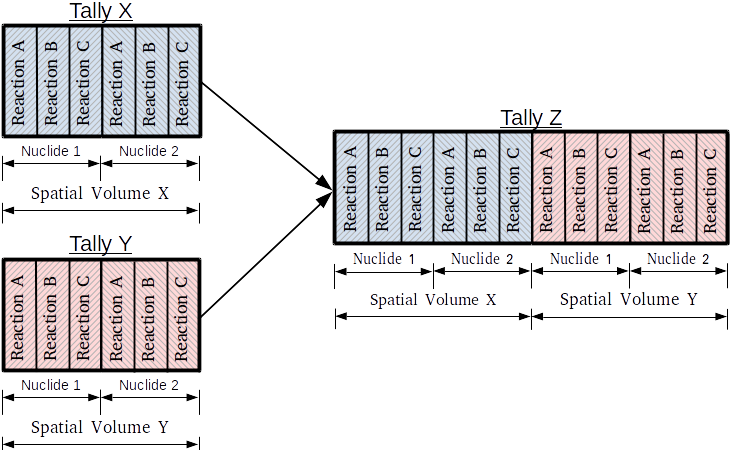
\includegraphics[width=0.6\linewidth]{figures/tally-merge}
  \caption{}
\end{subfigure}
\begin{subfigure}{\textwidth}
  \centering
  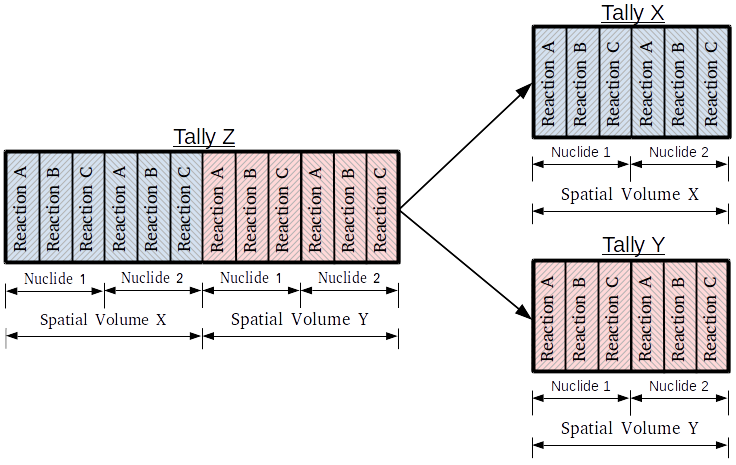
\includegraphics[width=0.6\linewidth]{figures/tally-slice}
  \caption{}
\end{subfigure}
\caption{Two \texttt{Tally} objects for different spatial volumes are merged into a single \texttt{Tally} (a). A single \texttt{Tally} is sliced by spatial volume into two distinct \texttt{Tally} objects (b).}
\label{fig:tally-merge-slice}
\end{figure}

%%%%%%%%%%%%%%%%%%%%%%%%%%%%%%%%
\subsubsection{Tally Arithmetic}
\label{subsubsec:tally-arithmetic}

A variety of reaction rate and flux tallies must be arithmetically combined in order to compute MGXS with Monte Carlo. At the most general level, a reaction rate tally must be divided by a flux tally for each energy group, nuclide and tally volume. The Python API provides a novel feature known as \emph{tally arithmetic} to enable arithmetic combinations of tallies with efficient vectorized numerical operations across energy groups, nuclides and spatial tally zones.

Tally arithmetic is an object-oriented data processing feature that arithmetically combines two or more tallies and/or scalar values into new \emph{derived tallies}. The Python API overloads the \texttt{Tally} class' operators for addition, subtraction, multiplication and division. Furthermore, the \texttt{Tally} class supports summation and averaging operations across some or all of its filter, nuclide or score bins.

Multi-group cross sections may be simply and efficiently computed with tally arithmetic. For example, the following code snippet illustrates how tally slicing and arithmetic are used to compute a total MGXS. The total MGXS that is returned from the tally division operation is encapsulated within a \texttt{Tally} object. This is the approach used by the MGXS generation module created for OpenMC.

\lstinputlisting[language=Python, basicstyle=\ttfamily\scriptsize, caption={MGXS calculation with tally arithmetic.}, label={lst:python-input}]{listings/tally-arithmetic.py}

Tally arithmetic automatically propagates the uncertainties of the tally operands through the arithmetic operation to estimate the uncertainty of the resulting derived tally. Estimates of the variance for derived tallies are deduced from standard error propagation theory~\cite{bevington2003data}. The division operator is primarily used to to compute MGXS from MC tallies. Consider two random variables $X$ and $Y$, generated from distributions with variances $\sigma_{X}^2$ and $\sigma_{Y}^2$, that are divided into a new random variable $Z$ with variance $\sigma_{Z}^2$:

\begin{equation}
\label{eqn:div-prop}
\sigma_{Z}^{2} \approx Z^{2}\left[\left(\frac{\sigma_{X}}{X}\right)^{2} + \left(\frac{\sigma_{Y}}{Y}\right)^{2} - 2\frac{\sigma_{XY}}{Z}\right]
\end{equation}

\noindent The variables $X$ and $Y$ may correspond to reaction rates and the flux tallies, while $Z$ could correspond to the MGXS.

The covariance $\sigma_{XY}$ is not generally computable using the standard formulation for a tally estimator in a Monte Carlo simulation. Although it would be possible to estimate the covariance using ensemble statistics, this is typically infeasible. Instead, the covariance term in \cref{eqn:div-prop} is currently neglected by OpenMC's implementation of tally arithmetic. In general, the random variables for reaction rates and fluxes in the same volume of phase space are highly correlated, such that a conservative estimate of the variance for MGXS is obtained by neglecting the covariance.

%%%%%%%%%%%%%%%%%%%%%%%%%%%%%%%%%%%%%
\subsection{Distributed Cell Tallies}
\label{subsec:distribcells}

%Many Monte Carlo codes, including OpenMC, use some variant of combinatorial geometry (CG) because it can represent arbitrary, repeating geometries such as fuel pins and assemblies. However, the CG approach is challenged by applications which require tallies in each instance of a repeated cell throughout a reactor geometry. The ``brute force'' solution is to instantiate a unique cell for each distinct tally zone. However, this defeats the purpose of using CG for its compact representation, and it is not scalable to problems with large tally datasets such as those considered in this thesis.

The \emph{distributed cell tally} algorithm was implemented in OpenMC \cite{lax2014distribcell} to permit simply defined spatial tally zones across repeated cell instances. The distributed cell tally algorithm -- abbreviated as the \emph{distribcell} algorithm -- may be used to compute spatially-varying MGXS across fuel pin cell instances. The distribcell algorithm classifies each unique cell instance using a process that consumes orders of magnitude less memory than would be required by the ``brute force'' approach necessary to accomplish the same objective with other commonly used Monte Carlo codes. Only a single transparent line of XML input is necessary to define a distribcell tally that may span across an arbitrary number of instances for a particular cell. Furthermore, the Python API may be used to perform efficient vectorized transformations of distribcell tally data stored as contiguous NumPy arrays to compute MGXS.
